
\subsection{Methods 2.6.1 The direct contribution of thrombolysis use to the shift in probability of a good outcome}

The model using the definition of mRS 0-1 as a good outcome matched the definition used in the meta analysis of clinical trials \cite{emberson_effect_2014}. 


%%%%%%%%%%%% 3.6.3  %%%%%%%%%%%%%%%%%
\subsubsection{The direct contribution of thrombolysis use to the shift in probability of a good outcome}

Using the counterfactual results for all of the patients in the first k-fold test set that received thrombolysis, figure \ref{fig:shap_shift_lvo_nlvo} shows a linear regression fitted to the shift in the contribution from receiving thrombolysis towards having a good outcome at discharge (mRS0-1) with respect to the onset to thrombolysis time. 

Figures \ref{fig:stats_table_common_odds_ratio} and \ref{fig:stats_table_mrs1} show that the logistic regression coefficients are statistically significant. Taking mRS 0-1 as a good outcome, we found that the effect of thrombolysis had declined to zero at 328 minutes, and the effect from thrombolysis was improving odds of a good outcome by 0.90 if it were, theoretically, given at the time of stroke onset. Figure \ref{fig:shap_shift_lvo} shows results for the patient cohort with a stroke severity NIHSS 11+ (used as a surrogate to identify a large vessel occlusion). Figure \ref{fig:shap_shift_nlvo} shows results for the patient cohort with a stroke severity NIHSS 0-10 (used as a surrogate to identify a non-large vessel occlusion). Linear regression coefficients in both groups were statistically significant (figures \ref{fig:stats_table_common_odds_ratio} and \ref{fig:stats_table_mrs1}). We observed that the maximum theoretical effect of thrombolysis (if given at time of stroke onset) was greater for the LVO surrogate group (1.048 log odds for mRS0-1) than the non-nLVO surrogate group (0.771 log odds for mRS0-1). However the effect of thrombolysis declined a little faster in the LVO-surrogate group (reaching no effect at 314 minutes for LVO-surrogate patients, compared to 351 minutes for nLVO-surrogate patients).

A secondary analysis (reported in the supplementary material) repeated this analysis using the full log-odds change in achieving a given mRS threshold with and without. Using the full model prediction, rather than isolating the effect of thrombolysis using thrombolysis SHAP, produced similar results, but with a little larger predicted effect of thrombolysis (e.g  maximum theoretical beneficial of thrombolysis of improving the log odds of being discharged mRS 0-2 of 1.1 (\textit{c.f.} 0.90 when using the isolated effect of thrombolysis from the thrombolysis SHAP values, with no-effect time being 328 minutes and 334 minutes for the isolated and full effect models).

\begin{figure}[!ht]
    \centering
    \begin{subfigure}[b]{1\textwidth}
      \centering
      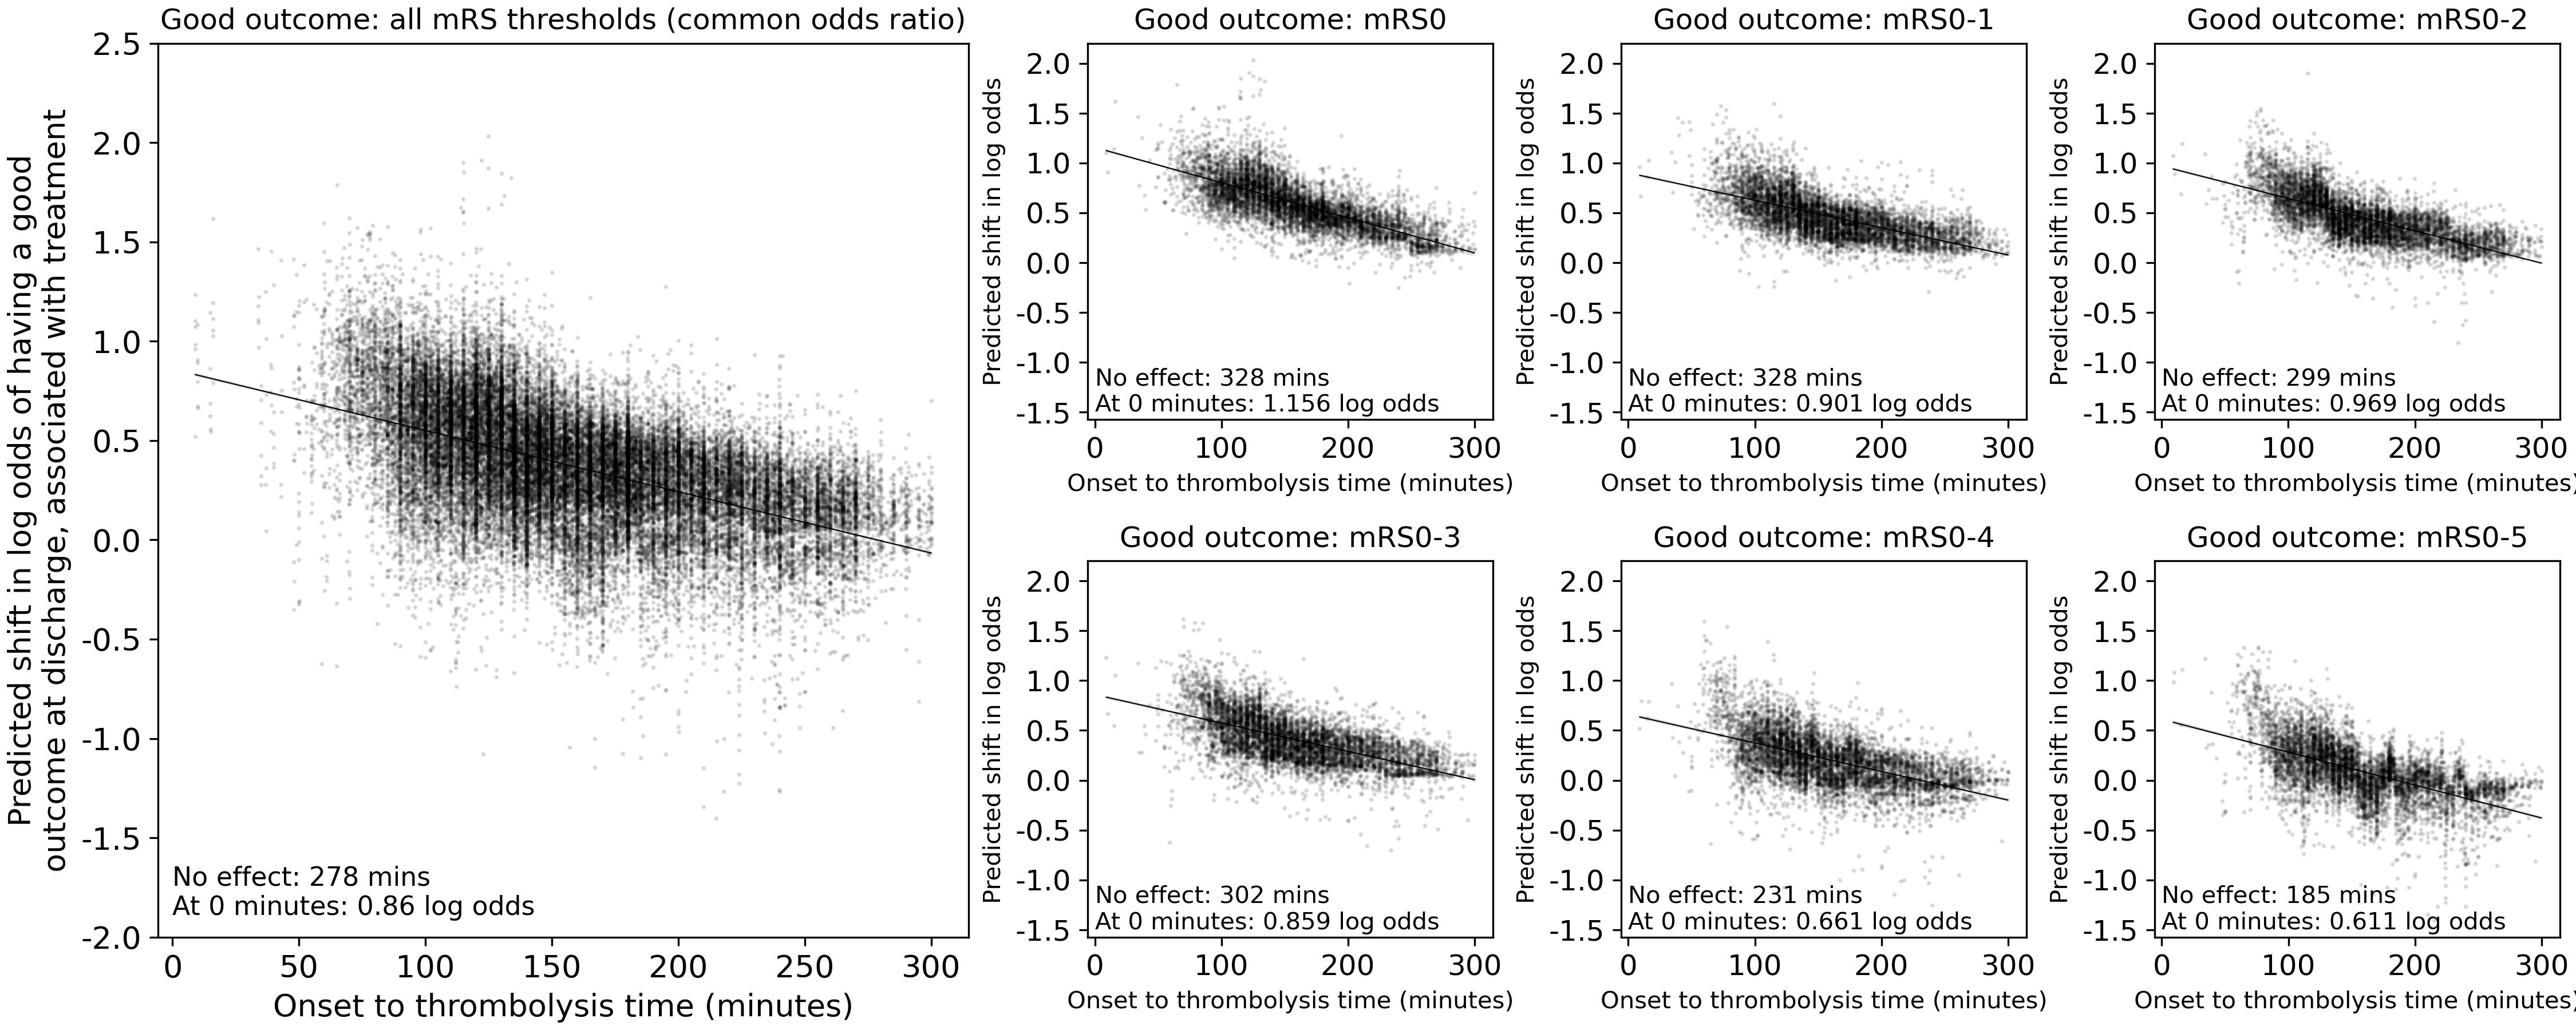
\includegraphics[width=1\textwidth]{./images/103_xgb_7_features_1fold_binary_improvement_logodds_bymRSthreshold_sns_subplots_nLVO_LVO_ivt_shap_paper}\\
      \caption{Patients in the test set that received thrombolysis}
      \label{fig:shap_shift_lvo_nlvo}
    \end{subfigure}
    \hfill
    \begin{subfigure}[b]{1\textwidth}
      \centering    
      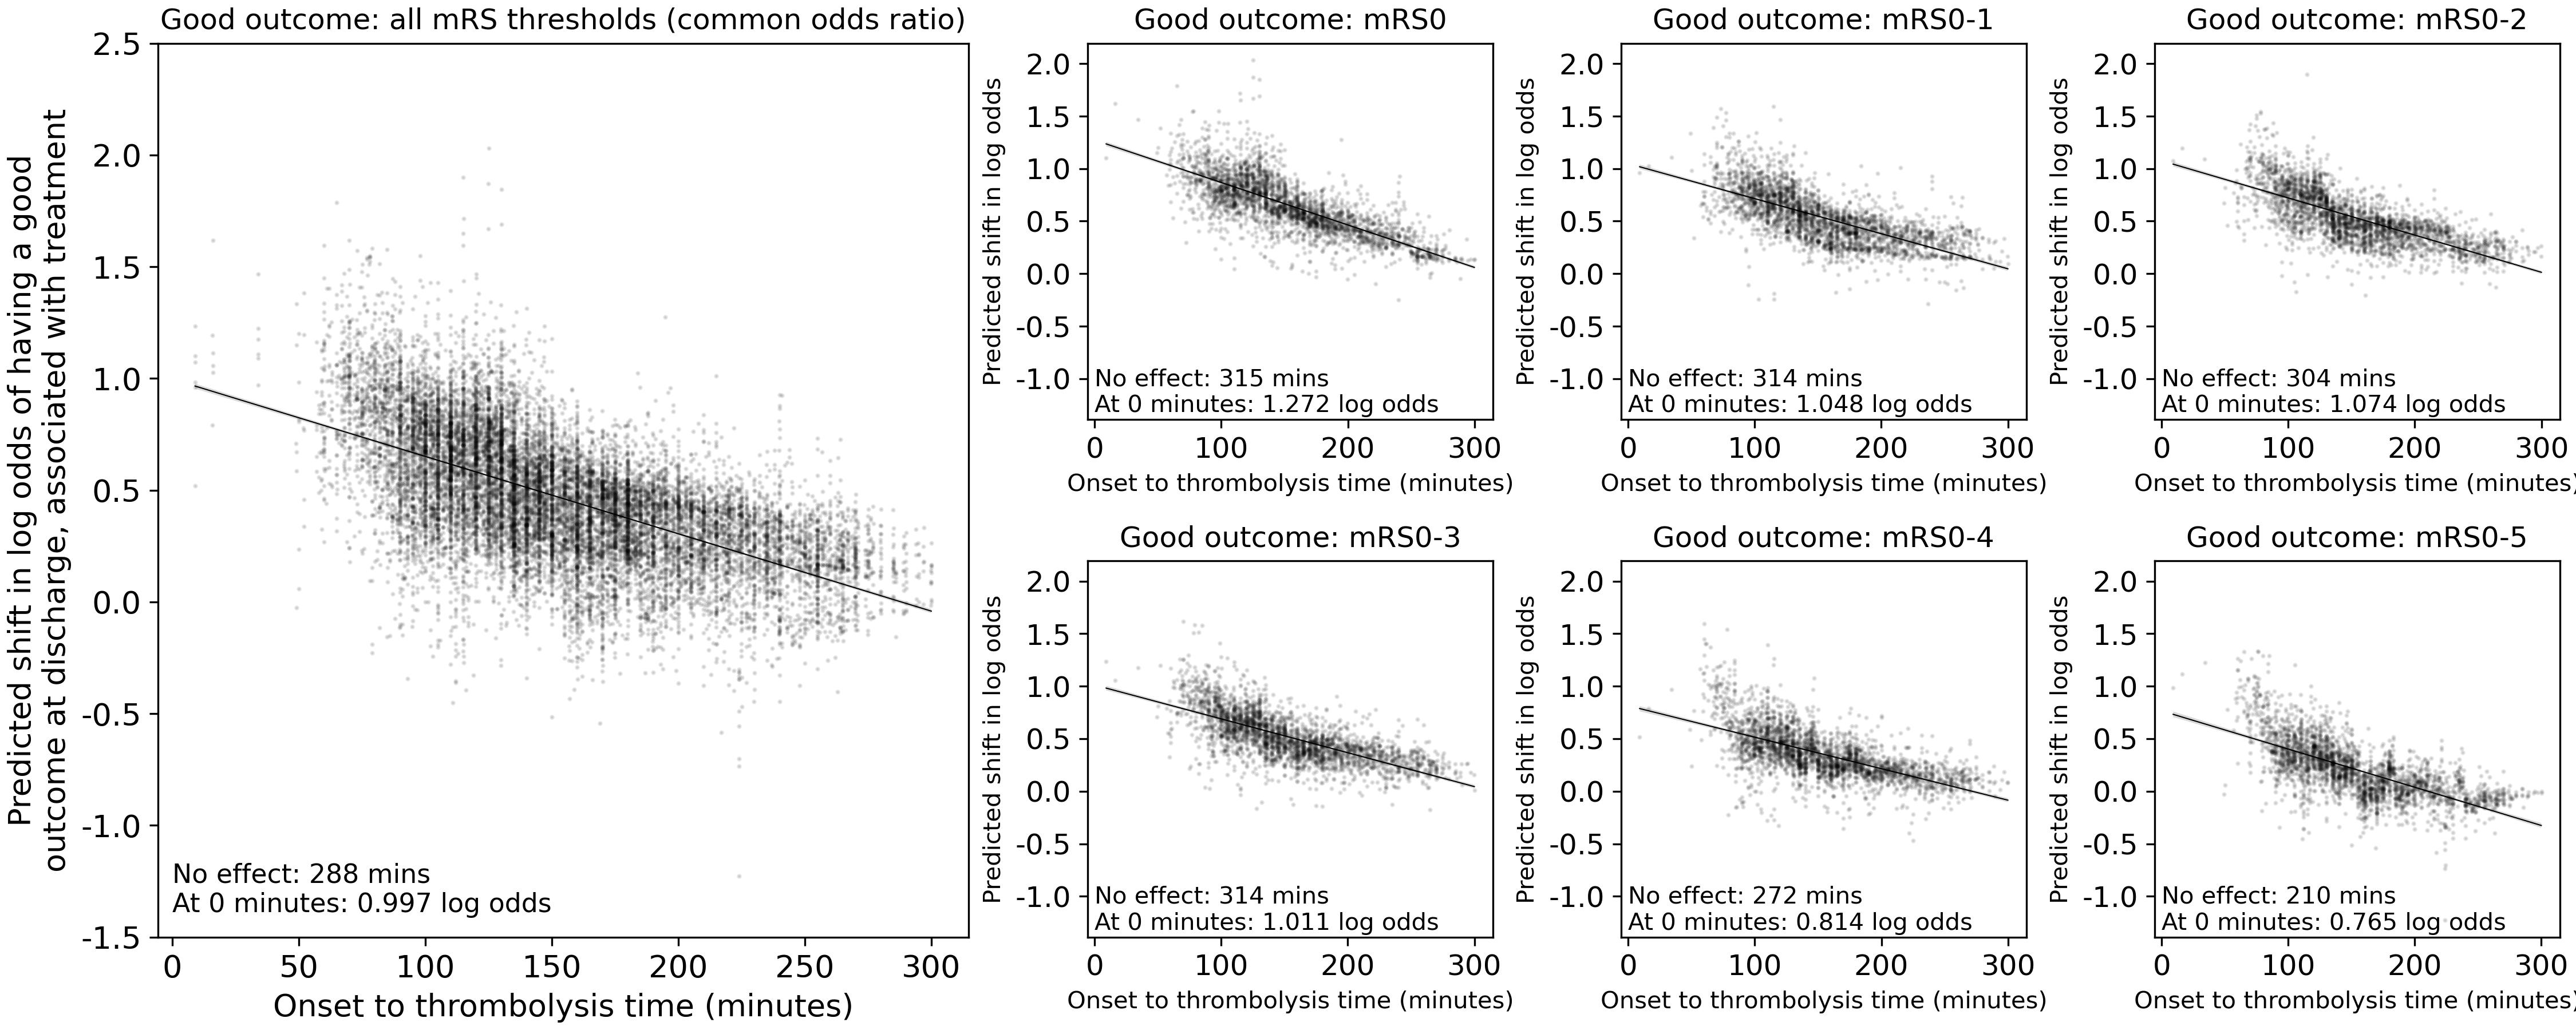
\includegraphics[width=1\textwidth]{./images/103_xgb_7_features_1fold_binary_improvement_logodds_bymRSthreshold_sns_subplots_LVO_ivt_shap_paper}\\
      \caption{Patients in the test set that received thrombolysis with NIHSS 11+ (surrogate for selecting patients with a LVO)}
      \label{fig:shap_shift_lvo}
    \end{subfigure}
    \hfill
    \begin{subfigure}[b]{1\textwidth}
      \centering
      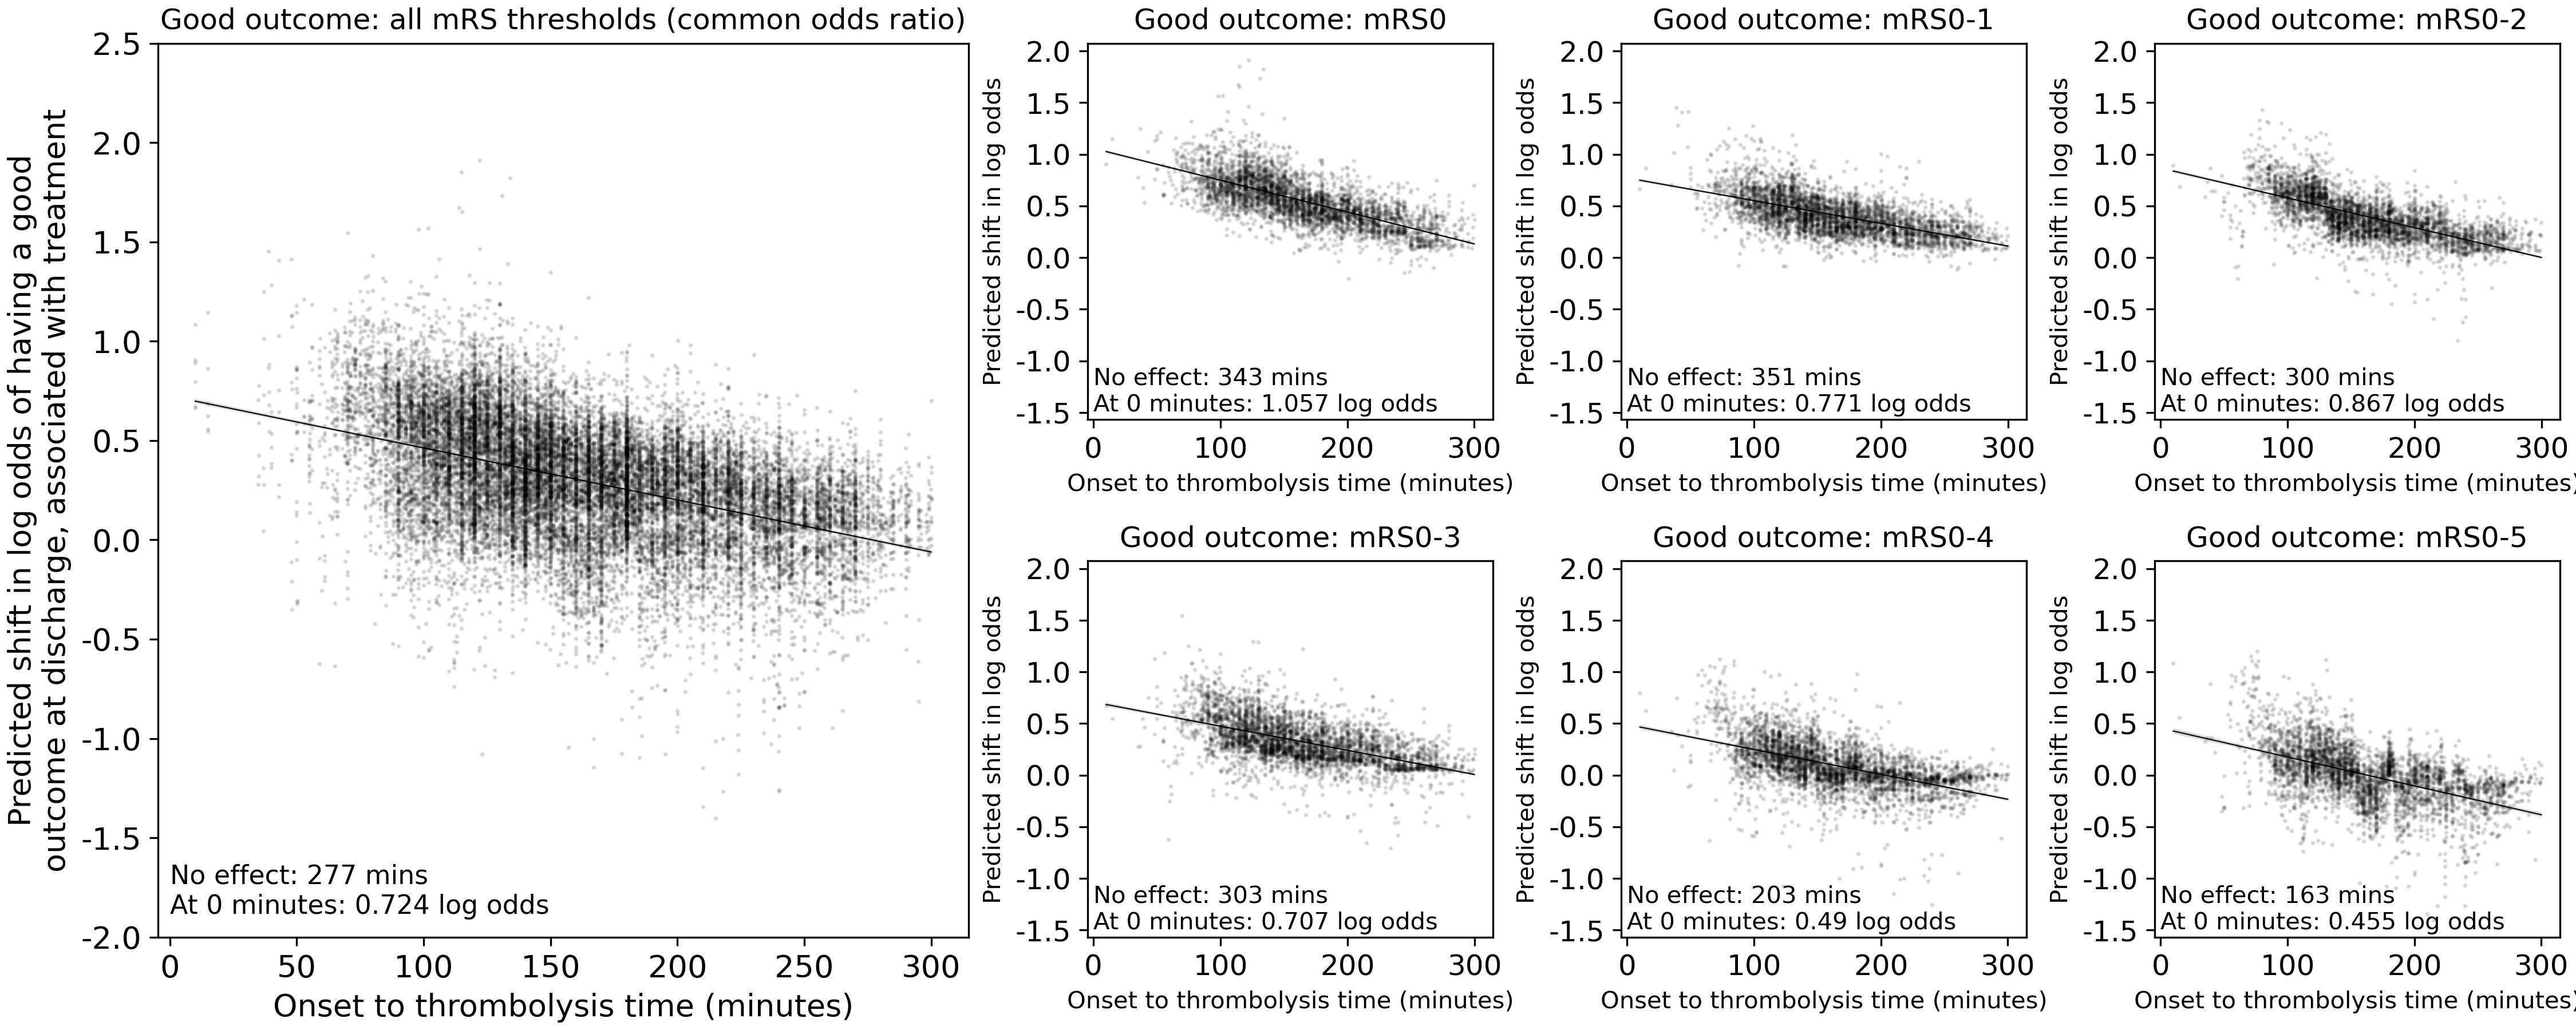
\includegraphics[width=1\textwidth]{./images/103_xgb_7_features_1fold_binary_improvement_logodds_bymRSthreshold_sns_subplots_nLVO_ivt_shap_paper}\\
      \caption{Patients in the test set that received thrombolysis with NIHSS 0-10 (surrogate for selecting patients with a nLVO)}
      \label{fig:shap_shift_nlvo}
    \end{subfigure}
    \label{fig:shap_shift}
    \caption{Fitting logistic regression to the shift in the contribution from receiving thrombolysis towards having a good outcome at discharge with respect to the onset to thrombolysis time. A subplot for each mRS threshold used to define a good outcome.}
\end{figure}



%%%%%%%%%%%%%%%%%%%%%%%%%%%%%%%%%%%%%%%%%%%5555





For all thresholds

\begin{figure}[!h]
    \begin{subfigure}[b]{1\textwidth}
    \centering
        \begin{tabular}{llllllll}
        \toprule
        Variables & coef & std err & t & P$>$$|$t$|$ & [0.025 & 0.975] \\ \midrule
        const  & 0.7732 & 0.004 & 185.552 & 0.000 & 0.765 & 0.781\\
        onset\_to\_thrombolysis\_time & -0.0027 & 2.47e-05 & -107.434 & 0.000 & -0.003 & -0.003\\
        \bottomrule
        \end{tabular}
      \caption{LVO and nLVO}
      \label{fig:stats_table_lvo_nlvo}
    \end{subfigure}
%    \hfill
%    \hfill

    \vspace{15mm}
    \begin{subfigure}[b]{1\textwidth}
      \centering    
        \begin{tabular}{llllllll}
        \toprule
        Variables & coef & std err & t & P$>$$|$t$|$ & [0.025 & 0.975] \\ \midrule
        const    &                      0.8645  &    0.005 &   161.438  &    0.000    &   0.854   &    0.875\\
        onset\_to\_thrombolysis\_time   & -0.0027  &  3.3e-05 &   -83.259  &    0.000   &   -0.003    &  -0.003\\
        \bottomrule
        \end{tabular}
      \caption{LVO only}
      \label{fig:stats_table_lvo}
    \end{subfigure}
%    \hfill

    \vspace{15mm}
    \begin{subfigure}[b]{1\textwidth}
      \centering
       \begin{tabular}{llllllll}
        \toprule
        Variables & coef & std err & t & P$>$$|$t$|$ & [0.025 & 0.975] \\ \midrule
        const                   &       0.6723 &     0.006 &   115.617 &     0.000 &      0.661  &     0.684\\
        onset\_to\_thrombolysis\_time  &  -0.0024 &  3.37e-05 &   -70.894  &    0.000 &     -0.002  &    -0.002\\
        \bottomrule
        \end{tabular}
        \caption{nLVO only}
      \label{fig:stats_table_nlvo}
    \end{subfigure}
    \label{fig:stats_table}
\end{figure}











For the threshold mRS0-1



\begin{figure}[!h]
    \begin{subfigure}[b]{1\textwidth}
    \centering
        \begin{tabular}{llllllll}
        \toprule
        Variables & coef & std err & t & P$>$$|$t$|$ & [0.025 & 0.975] \\ \midrule
        const            &              0.9012  &    0.007  &  132.519   &   0.000  &     0.888  &     0.915\\
        onset\_to\_thrombolysis\_time  &  -0.0027  & 4.04e-05  & -68.058  &    0.000   &   -0.003   &   -0.003    \\    \bottomrule
        \end{tabular}
      \caption{LVO and nLVO}
      \label{fig:stats_table_lvo_nlvo_mrs1}
    \end{subfigure}
%    \hfill
%    \hfill



    \vspace{15mm}
    \begin{subfigure}[b]{1\textwidth}
      \centering    
        \begin{tabular}{llllllll}
        \toprule
        Variables & coef & std err & t & P$>$$|$t$|$ & [0.025 & 0.975] \\ \midrule
        const                  &        1.0476  &    0.011  &   96.746  &    0.000   &    1.026 &      1.069\\
        onset\_to\_thrombolysis\_time  &  -0.0033 &  6.67e-05  &  -50.042   &   0.000  &    -0.003   &   -0.003\\
        \bottomrule
        \end{tabular}
      \caption{LVO only}
      \label{fig:stats_table_lvo_mrs1}
    \end{subfigure}
%    \hfill


    \vspace{15mm}
    \begin{subfigure}[b]{1\textwidth}
      \centering
       \begin{tabular}{llllllll}
        \toprule
        Variables & coef & std err & t & P$>$$|$t$|$ & [0.025 & 0.975] \\ \midrule
        const               &           0.7708 &     0.008   &  97.613 &     0.000 &      0.755 &      0.786\\
        onset\_to\_thrombolysis\_time  &  -0.0022 &   4.57e-05 &    -48.109    &  0.000   &   -0.002   &   -0.002\\
        \bottomrule
        \end{tabular}
        \caption{nLVO only}
      \label{fig:stats_table_nlvo_mrs1}
    \end{subfigure}
    \label{fig:stats_table_mrs1}
\end{figure}

The results from the set of six models, therefore, reports a cumulative probability distribution across the seven mRS levels for each patient. 

\textit{Good outcome} model [target feature: patients disability level at discharge is at or below the specified mRS score]: Fit a logistic model to predict the likelihood of being below a specified disability at discharge for each patient who had a stroke. 

Machine models are used to predict the likelihood of a patient with a stroke having a disability level at discharge less than a specified threshold.


\textbf{KP WANT TO INCLUDE "within 400 minutes"} for the shift in probability six subplots?



EXTRA TEXT: \textit{Models can be used to explore the predicted outcome for counterfactual cases, for our case we are interested in exploring the predicted outcome for patients had they not received thrombolysis. This is achieved by setting the feature value for onset to thrombolysis time to 999999 minutes.}


No effect (0 log odds) at 328 minutes. Max effect (0.9 log odds) at 0 minutes




\textit{Introduction}:
This work aims to understand the effect of thrombolysis on the likelihood of a good outcome at discharge for patients with an ischaemic stroke in England and Wales, using observational data.\\
Patients:
A total of 168,347 patients with an ischaemic stroke who arrived by ambulance at all 118 emergency stroke hospitals in England and Wales that did not go on to have thrombectomy, from 2016 to 2021 (inclusive).\\
\textit{Methods}:
Machine learning was applied to the Sentinel Stroke National Audit Programme data set, to learn the effect that thrombolysis has on the likelihood of a patient having a good outcome at discharge. We used XGBoost machine learning models, coupled with a SHAP model for explainability; Shapley (SHAP) values, providing estimates of how patient features, pathway durations, treatment decisions and hospital identity, influence the odds of a good outcome. We define a good outcome as being below a specified modified Rankin Scale (mRS) level. We train a set of six individual models, each using a different level of mRS as the threshold ($<$= mRS0, $<$= mRS1, $<$= mRS2, $<$= mRS3, $<$= mRS4, and $<$= mRS5).\\
\textit{Results}:
Analysis on the observational dataset shows that maximum improvement of being discharged with a good outcome (defined as mRS0-1) from receiving thrombolysis occurs when treatment is given at the time of onset: 0.901 log odds (2.46 odds, 71.1\% probability). The level of improvement from thrombolysis reduces over time, with no effect occurring at 328 minutes (5.5 h).\\
\textit{Conclusions}:
Using explainable machine learning on observational data, we have seen that the effect of thrombolysis on a patient having a good outcome at discharge (mRS0-1) is comparable to the result from the meta analysis of the clinical trials: 0.693 log odds (2 odds, 74.3\% probability) at 0 minutes, with no effect at 378 minutes (6.3 h).

Condensed:
This study examines the impact of thrombolysis on discharge outcomes for ischemic stroke patients in England and Wales using observational data from 168,347 patients across 118 emergency stroke hospitals from 2016 to 2021. The research employs machine learning techniques, specifically XGBoost models with SHAP for explainability, to analyze the Sentinel Stroke National Audit Programme dataset.
The study defines a good outcome based on modified Rankin Scale (mRS) levels, training six models with different mRS thresholds. Results show that thrombolysis has the greatest benefit when administered at stroke onset, improving the odds of a good outcome (mRS0-1) by 0.901 log odds (2.46 odds, 71.1\% probability). This effect diminishes over time, becoming negligible at 328 minutes (5.5 hours) post-onset.
The findings from this observational data analysis align closely with meta-analyses of clinical trials, which report a 0.693 log odds improvement (2 odds, 74.3\% probability) at 0 minutes, with no effect after 378 minutes (6.3 hours). This study demonstrates the potential of applying explainable machine learning to observational data for understanding stroke treatment outcomes.




For the feature \textit{onset to thrombolysis time} (which contains the duration of the entire pathway, and uses the value 999999 to represent no thrombolysis), 
SHAP values can be assessed locally (at patient level) and globally (at patient cohort level to understand general patterns of how outcomes with and without thrombolysis differ by patient characteristics).



Fit a logistic regression to the improvement in log odds of a good outcome with respect to the onset to thrombolysis time. Figure \ref{fig:shap_shift_lvo_nlvo} shows data for all patients that receive thrombolysis in the test set. Taking mRS0-1 as a good outcome, we see that from our observational data there is no effect of thrombolysis at 328 minutes, and maximum effect from thrombolysis is 0.9 if it is given at time of stroke onset. Figure \ref{fig:shap_shift_lvo} shows data for all patients with a stroke severity NIHSS 11+ (used as a surrogate to identify a large vessel occlusion) that receive thrombolysis in the test set. Figure \ref{fig:shap_shift_lvo_nlvo} shows data for all patients with a stroke severity NIHSS 0-10 (used as a surrogate to identify a non large vessel occlusion) that receive thrombolysis in the test set.


***









\section{extra words}

From Motivation
Regardless of the efforts spent, the rates have not changed and, nationally, the 20\% target has never been met. 

It has Even accounting for  found The barrier to increasing the thromboylsis rates are that it comes with it's risks. If it does not kill you (by causing a catastrophic bleed) then you will likely have a less severe disability (due to breaking down the clot and restoring blood flow to the brain sooner).

In addition, during communications with individual stroke teams, it became apparent that clinicians had a varied range of enthusiasm levels to giving thrombolysis. This can be based on the culture of the hospital, and informed by the previous experience of administering the drug.

A study on a single acute stroke hospital in SW England identified that pathway speed was a barrier [2014, Toms work]. Thrombolysis needs to be administered within 4 hours of stroke onset, so that the benefit (breaking down the clot and restoring blood flow to the brain) still outweighs the risks (causing a catastrophic bleed). The suggested change, for increasing the thrombolysis rates at this hospital, was to call the stroke team ahead from the ambulance so that the stroke team could prepare for the patient arrival, thus reducing the duration taken from arrival to treatment. This translated into an increase in thrombolysis rates from n\% to n\%.

This insight was rolled out across all of the hospitals in the region (SW England) [2016 (me and MA)]. It was anticipated that for each hospital a specific part of the pathway speed would be identified as the main barrier to receive. However, in addition to pathway speed, it was observed that differences in staff behaviour affected the thrombolysis rates. For example, some stroke teams will put extra “detective work” to estimate the stroke onset, when other teams will take it as written if someone says “I don’t know when the stroke started”, thus removing the possibility of considering thrombolysis for that patient. 

We have looked at the acute stroke pathway (on an individual hospital level) to try to identify the barriers at a hospital level. We identified that it was not all down to the speed of the pathway, it was also due to personal behaviours (around obtaining the onset time, and also the clinical decision to treat). Some hospitals were just more enthusiastic at giving thrombolysis, whereas others were more cautious.

To explore this variety in decision making, and in an attempt to identify additional patients that hospitals could consider giving thrombolysis to (with the motivation to help to increase the thrombolysis rates to the national target of 20\%), we looked at the effect of rolling out the "high benchmark thrombolysis decision" across all hospitals. The "high benchmark thrombolysis decision" was predicting what the treatment decision would be at the 25 hospitals with the most willingness to give treatment. The main resistance this work met, from both patients and clinicians from the lower thrombolying hospitals, was that how do we know if the high benchmark hospitals are making the correct decision based on patient outcomes.

Since YEAR SSNAP has been collecting data on the patients disability at discharge, recorded as the modified Rankin Scale (mRS). This feature is complete for n\% of patients.

Using this feature, we look to address the question that kept coming our way: "What is the best treatment for the patient"? We can now model at a hospital level, and instead of rolling out the "high benchmark thrombolysis decision" we can roll out the thrombolysis decision that's best for the patient, and analyse the thrombolysis rates that this will obtain.

NHS England has a target of 20\% thrombolysis rates. Currently have range 3\% to 30\%.

Lots of work and effort has gone into trying to increase the rates to reach the national target, which have not succedded in many years - ?? years after the clinical trial meta analysis the rates have not changed??.

The barrier to increasing the thromboylsis rates are that it comes with it's risks. If it does not kill you (by causing a catastrophic bleed) then you will likely have a less severe disability (due to breaking down the clot and restoring blood flow to the brain sooner).

Clinicians therefore have a different enthusiasm to giving this treatment which can be based on the culture of the hospital, and informed by the previous experience of administering the drug.

We have looked at the acute stroke pathway (on an individual hospital level) to find ways of improving it to increase the thromboylsis rates. Wanted to identify the barriers at a hospital level. We identified that it was not all down to the speed of the pathway, it was also due to personal behaviours (around obtaining the onset time, and also the clinical decision to treat). Some hospitals were just more enthusiastic at giving thromboblyisis, and others were more cautious.

To explore this variety in decision making, and in an attempt to identify additional patients that hospitals could consider giving thrombolysis to (with the motivation to help to increase the thrombolysis rates to the national target of 20\%), we looked at the effect of rolling out the "high benchmark thrombolysis decision" across all hospitals. The "high benchmark thrombolysis decision" was predicting what the treatment decision would be at the 25 hospitals with the most willingness to give treatment. The main resistance this work met, from both patients and clinicians from the lower thrombolysing hospitals, was that how do we know if the high benchmark hospitals are making the correct decision based on patient outcomes.

Since YEAR SSNAP has been collecting data on the patients disability at discharge, recorded as the modified Rankin Scale (mRS). This feature is complete for n\% of patients.

Using this feature, we look to address the question that kept coming our way: "What is the best treatment for the patient"? We can now model at a hospital level, and instead of rolling out the "high benchmark thrombolysis decision" we can roll out the thrombolysis decision that's best for the patient, and analyse the thrombolysis rates that this will obtain.

\subsection{\textit{Threshold outcome} model}

\emph{Method}
\textit{Threshold outcome} model [target feature: below a specific mRS threshold at discharge]: A set of binary threshold models to predict whether the disability level on discharge for a patient is at or below each of the mRS levels. 

\emph{Results}
An alternative way to interpret the contributions of each feature to the prediction of a patients discharge disability is to analyse the SHAP values from the \textit{Threshold outcome} model (a set of six binary XGBoost models to predict whether a patient is at least as well as mRS0, mRS1, mRS2. mRS3. mRS4 and mRS5). A positive SHAP value for this model can always be interpreted as contributing to the patient having a more favourable outcome.

\begin{figure}
\subfloat[]{\includegraphics[width = 5in]{./images/080_shap_violin.png}}\\
\caption{}
\end{figure}

\begin{figure}
\subfloat[]{\includegraphics[width = 5in]{./images/080_shap_histogram.png}}\\
\caption{}
\end{figure}



DATA
Of these patients, ??? arrived within 4h of known stroke onset, and were used in this modelling study. A 4h onset-to-arrival cut-off was used to allow for 30min for scan and thrombolysis to be within the allowed 4.5 onset-to-thrombolysis time.


 This model has two parts:
\begin{enumerate}
    \item For the cohort of patients that were predicted to have a better outcome with treatment, 0 is they did not receive treatment, and 1 is they did receive treatment.
    \item For the cohort of patients that were predicted to not have a better outcome with treatment, 0 is they did receive treatment, and 1 is they did not receive treatment.
\end{enumerate}



\subsection{Feature selection}
 – those that sequentially lead to the most improvement in ROC AUC score to predict the patients disability level at discharge. 

The full dataset contains 55 features. In order to simplify the model (for enhanced explainability) we selected a subset of these features to be included in the machine learning model. Features were selected by forward-feature selection (using the k-fold model), identifying one feature at a time that led to the greatest improvement in accuracy as measured by the Receiver Operating Characteristic (ROC) Area Under Curve (AUC) (using the one vs rest approach for multi-0class classification models). We repeated this process, identifying the most important feature to add sequentially, until 25 features were selected. These results were used to identify the number of features to include in our machine learning models. We used the same set of features for the "made the correct treatment decision" model.

Using SHAP values, we revealed patient characteristics that contribute to a patient having the wrong treatment decisions.

We predicted which patients should receive thromboylsis based on whether treatment gave them a better outcome, which we defined (cautiously) as: 



\textit{Treatment decision matches predicted best treatment decision} model



Create two subpopulations based on whether the patient has a predicted better outcome with thrombolysis, and fit a separate model to each subpopulation to predict whether they received the matching treatment decision (where 0 represents not matching, and 1 represents matching).


\section{The Appendix containing further model accuracy analysis}

It is a well callibrated and reliable model.

\item Getting a prediction for having a better outcome with treatment.   

Use this model to predict the counterfactual for each patient (whether they did or did not receive IVT) to understand what impact has IVT had, and whether it was the best decision for that patient.

Using the two probability distributions for disability at discharge, can predict whether each patient has a better outcome receiving treatment. For those patients that received thrombolysis, set the feature onset to treatment time to -100 to predict what their disability at discharge probability is without treatment, and for those patients that were not given thrombolysis (hence do not have a scan to thrombolysis time recorded) assume it is the median of the attended hospital.


\textbf{Basing the paper on the story to get to this chart.}
Using this paper to help the flow: https://journals.sagepub.com/doi/full/10.1177/23969873231189040


This model is used to predict the counterfactual outcome for each patient (whether they did, and did not, receive thrombolysis). For those patients that received thrombolysis, create the counterfactual case by setting the feature onset to treatment time to -100 (to predict what their disability at discharge probability is without treatment). For those patients that were not given thrombolysis create the counterfactual case by assuming their scan to thrombolysis time (which is not recorded) is the median of the attended hospital, and set the feature onset to treatment time the sum of the pathway durations (onset to arrival [recorded], arrival to scan [recorded], scan to thrombolysis [median of attended hospital]). This gives two probability distributions for each patient: a probability across the range of mRS scores at discharge for when the patient receives thrombolysis; and another for not receiving thrombolysis. 

Using a cautious definition for what defines a better outcome with treatment: on average reduce disability, without increasing the risk of death and the severest disability (mRS5+), we can compare these two probability distributions for disability at discharge, and translate it into a binary feature for each patient to represent whether they are predicted to have a better outcome receiving thrombolysis.



SHAP methods section (removed words while threshold model not included in paper):
    2) a patient to have a disability beneath a mRS threshold on discharge, 3)....



\section{Words to describe the counterfactural method}
Using the two probability distributions for disability at discharge, can predict whether each patient has a better outcome receiving treatment. For those patients that received thrombolysis, set the feature onset to treatment time to -100 to predict what their disability at discharge probability is without treatment. For those patients that were not given thrombolysis (hence do not have a scan to thrombolysis time recorded) assume it is the median of the attended hospital.

For those patients that were not given thrombolysis create the counterfactual case by assuming their scan to thrombolysis time (which is not recorded) is the median of the attended hospital, and set the feature onset to treatment time the sum of the recorded pathway durations (onset to arrival and arrival to scan) and the median scan to thrombolysis time of the attended hospital.

Use \textit{Multiclass outcome} model to predict the probability distribution of the patients disability level at discharge for the counterfactual case: whether they did, or did not, receive thrombolysis. Use this to predict what impact receiving thrombolysis would have, and whether it was the best decision for that patient.





\begin{figure}[!h]
    \centering    
    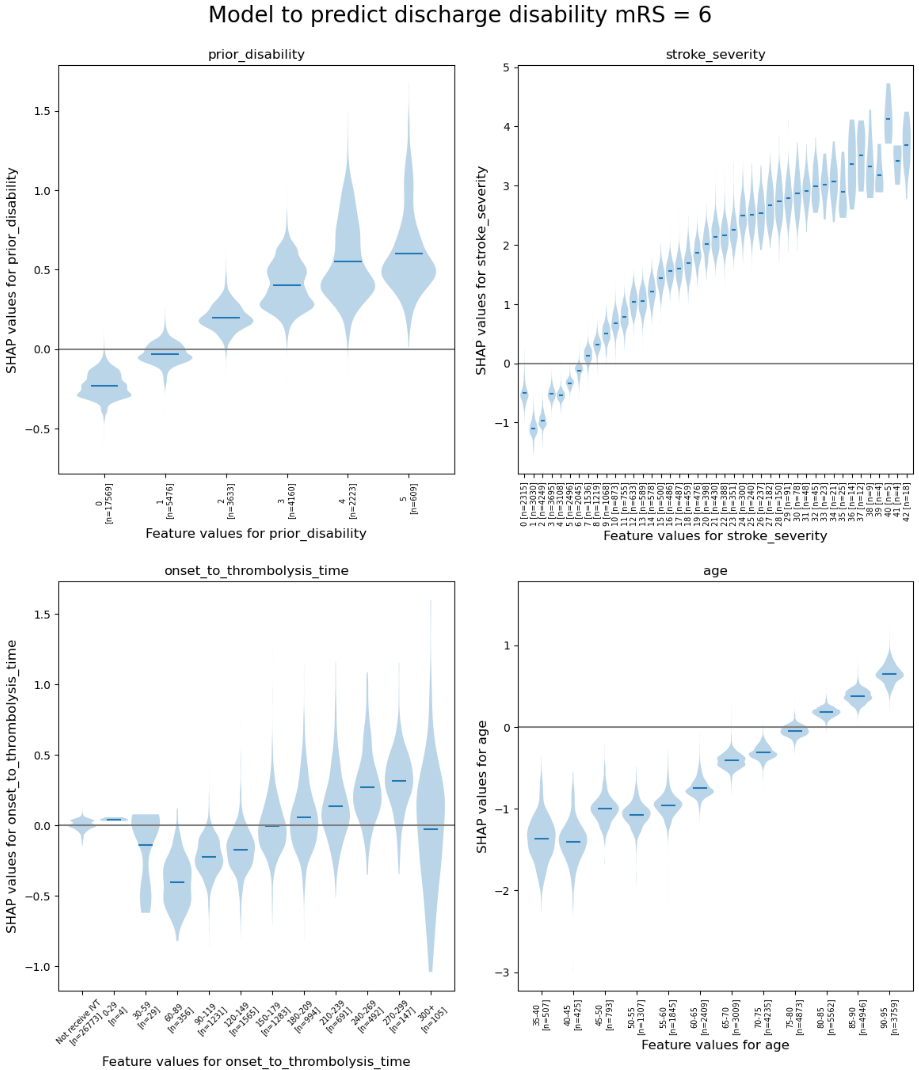
\includegraphics[width=0.75\textwidth]
    {./images/043_outcome_mrs6_violin_plots.png}\\
    \caption{}
    \label{fig:mrs6_violin}
\end{figure}

\begin{figure}[!h]
    \centering    
    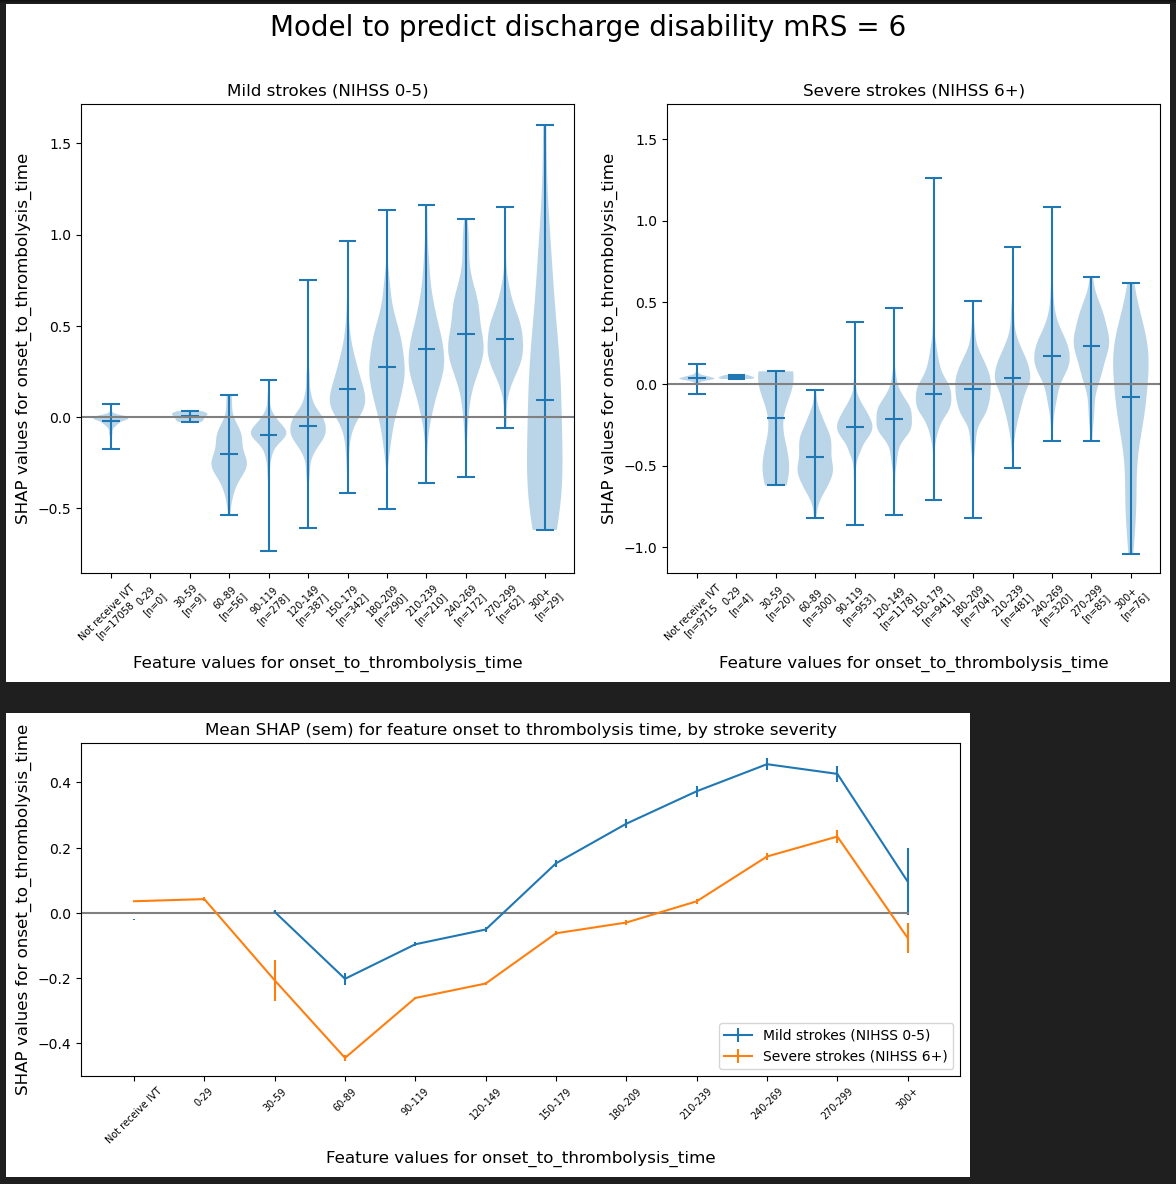
\includegraphics[width=0.75\textwidth]
{./images/053_predict_mrs6_split_by_ss.png}\\
    \caption{The impact of a feature value on the likelihood of death can be divided into subgroups. Here we see the effect of time to thrombolysis on likelihood of death for mild strokes (NIHSS0-5) and moderate and severe strokes (NIHSS 6+).}
    \label{fig:mrs6_violin_split}
\end{figure}


\section{results}
\subsection{feature selection}

A model with all features has average accuracy from 81.5\% to 90.6\% across the six models (standard deviation across the 5 kfolds ranged from 0.000 to 0.001). ROCAUC ranged from 0.894 to 0.935 (standard deviation across the 5 kfolds ranged from 0.000 to 0.001). 